\chapter{Generative Models and Networks}
\label{ch:Generative Models and Networks}\index{Generative Models and Networks}

\subsection{Definition}
A generative model \index{generative model} is an unsupervised statistical model that can be used to generate similar samples from the learning of observable examples \citep{shin:2017}.
These types of models make use of Naive Bayes rules in joint probability to calculate equation \ref{p(y,x)}:

\begin{equation}\label{p(y,x)}
p(y,x) = p(x)p(y|x)
\end{equation}

With \textit{x} being the input feature and \textit{y} being the given class \citet{ng:2002}.

Generative models are a concept which are currently limited in use due to the challenge of productively training them, 
where article such as \cite{goodfellow:2014} state the difficulty of 
finding the best way to train them as the probabilistic computation required tends to be hard to gather the linear units in a generative context.



They are still sought after due to their heavy use in computer vision such as image caption generation \citet{lin:2014,touretzky:1996}; projects related to speech and language for example speech synthesis \citet{ou:2012} and conversation with dialogue generation \citet{sordoni:2015}. Generational models have the capability of data generation from the given sample with the understanding of the structure of the input data even without labels \citet{tu:2007}.


\begin{figure}
  \centering
  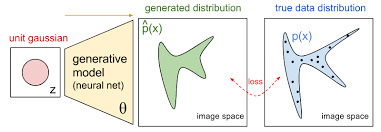
\includegraphics[width=1\linewidth]{graphics/generational_models/gm.png}
  \caption{The layout of a generative model that shows the production of a generated product that is a variation of the original image space. }
  \label{fig:GAN}
\end{figure}
\pagebreak
\section{Generative Adversarial Networks}

Generative Adversarial networks (GAN) are a type of generative approach that makes use of the creation of a network which consists of, the generator model which maps the latent space to the input space \textit{x} and with the introduction of a discriminative model. It will be used to classify the generated data sample of the first model and calculates the probability of the sample that it came from the product of the first model or the actual training data. These models  are trained simultaneously where the performance of the generative model is based on the probability of the discriminative model to make a mistake  \citet{goodfellow:2014}. \newline

GAN is defined by the following objective function:
\begin{equation}\label{minmax}
min_{D}max_{G} \ \ \ V(D,G)= \mathbf{E}_{x\textasciitilde pdata(x)}[log D(x)] + \mathbf{E}_{z\textasciitilde pz(z)} + [log(1 - D(G(z)))]

\end{equation}

Where \textit{D} is the discriminative model and is represented by a multilayered perceptron with parameters \textit{D(x; $\theta$d)} with a single scalar output. D(\textit{x}) is the probability that \textit{x}  came from the data rather than the output of \textit{G}, it represents the generative model which is also represented by a multilayered perceptron contains parameters $\theta$\textit{g}. The generator`s distribution \textit{pg} is learned by defining the input noise variables represented by \textit{pz(z)}. This is then represented by the data space as G(z;$\theta$g). The two models are trained simultaneously where \textit{D} is trained to maximize the probability of labelling the data \textit{`x`} as either if it came from the provided sample rather than from \textit{pg}, while \textit{G} is trained to minimize \textit{log(1-D(G(z)))}, therefore GANs follow a minmax game \citet{goodfellow:2014}.

\begin{figure}
  \centering
  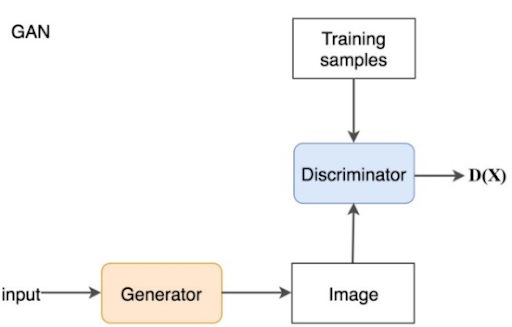
\includegraphics[width=1\linewidth]{graphics/generational_models/GAN.png}
  \caption{The components of a typical GAN system which includes a generative component that takes the dataset as inputs and the output is fed to the discriminator.  }
  \label{fig:GAN}
\end{figure}
\pagebreak
GANs is an area which can be used  for reinforcement learning in several different ways,one example is the learning of a conditional distribution for the generation of future possible states based on the current state of the samples and with hypothetical actions which can be taken as input \citet{goodfellow:2016}.


\section{Variational Autoencoders}

Variational Autoencoders are models that consist of neural networks of an encoder, a decoder with a loss function which can be trained using stochastic gradient descent. The encoder receives input data and produces a hidden representation of the same output with weight and biases. The encoder produces a latent vector space to lower the dimensionality space.
The decoder consists of another neural network where the input is the output of the encoder and the product of this network is the parameters of the probability distribution of the data with its constituent weights and biases. \citet{doersch:2016}.

\begin{figure}
  \centering
  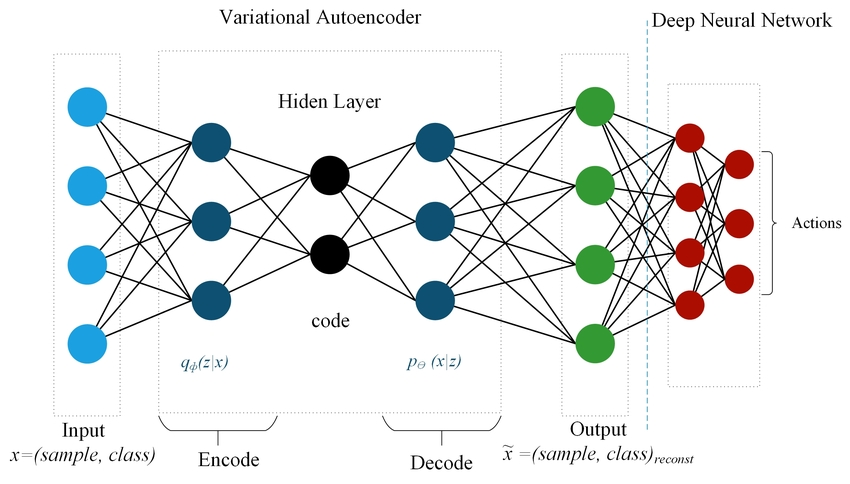
\includegraphics[width=1\linewidth]{graphics/generational_models/vae.png}
  \caption{The structure of a variational autoencoder that shows the process of encoding and decoding with the production of the output. }
  \label{fig:GAN}
\end{figure}

Variational Encoders have become a very popular approach to tackle distributions with unsupervised learning and these models have already proved to tackle complicated distributions by generating data of different kinds of projects \citet{doersch:2016}.

The article by \citet{jain:2017} works on the generation of diverse visual questions wrapped around given images, this can be used for educational systems to AI assistants such as chat bots, driving assistance or for self entertainment. The author of the article thinks that this type of task is important for the reason of that it is wrapped around similarly to 'future prediction' and that it will solve the task of visual question and answering.   

\pagebreak
\section{Boltzmann Machine}

A Boltzmann Machine is a type of stochastic recurrent neural network where it has a straightforward learning algorithm that provides the ability of using data sets that contain binary vectors to work out compelling features. They are heavily used to solve search problems where the dynamics of a Boltzmann machine allow the weights of a connection to be fixed so that they can represent the cost function of an optimization problem and binary state vectors will then be sampled to provide adequate solutions to the provided optimization problem \citet{hinton:2007}. 

The article by \citet{nie:2015} makes use of a generative restricted Boltzmann machine to be implemented and tested on two computer vision applications, mainly facial expression recognition and human action recognition. The model is made up of a Gaussian-Binary restricted Boltzmann machine to model high-dimensional motion data to obtain the likelihood of the model.

A Multimodal Deep Boltzmann machine was used in the article by \citet{srivastava:2012} for a series of experiments and its performance was compared with other classifiers. This generative machine works by having two types of Deep Boltzmann machines which each include a number of hidden layers that are interconnected with each other only. These two types of DBMs have their own functionality and they are linked together by a common layer that joins the image and text inputs. The task at hand was the classification of images that contain different tags according to the content of the image. The DBM outperformed other machine learning algorithms such as an SVM and even an Autoencoder which was based on the works by \citet{ngiam:2011} and even other deep learning methods for example deep belief networks.

Generative models are a highly researched and powerful way of understanding and training a model with the data distributed. Articles such as \citet{georghiades:2000} state how their results and performance surpass those of other state of the art models in the implementation of facial recognition in different orientations.  

